\documentclass[10pt]{standalone}
\usepackage{amsmath}
\usepackage{pgf,tikz}
\usepackage{mathrsfs}
\usetikzlibrary{arrows}
\pagestyle{empty}
\begin{document}
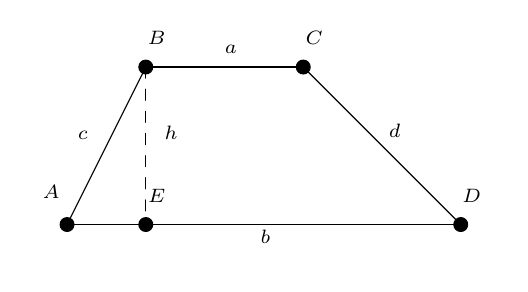
\begin{tikzpicture}[line cap=round,line join=round,>=triangle 45,x=1.0cm,y=1.0cm]
\clip(-1.5,-0.5) rectangle (4.5,2.5);
\draw (-1.,0.)-- (0.,2.);
\draw (0.,2.)-- (2.,2.);
\draw (2.,2.)-- (4.,0.);
\draw (4.,0.)-- (-1.,0.);
\draw [dash pattern=on 4pt off 4pt,color=black] (0.,2.)-- (0.,0.);
\begin{scriptsize}
\draw [fill=black] (-1.,0.) circle (2.5pt);
\draw[color=black] (-1.2,0.41) node {$A$};
\draw [fill=black] (0.,2.) circle (2.5pt);
\draw[color=black] (0.14,2.37) node {$B$};
\draw [fill=black] (2.,2.) circle (2.5pt);
\draw[color=black] (2.14,2.37) node {$C$};
\draw [fill=black] (4.,0.) circle (2.5pt);
\draw[color=black] (4.14,0.37) node {$D$};
\draw[color=black] (-0.8,1.13) node {$c$};
\draw[color=black] (1.08,2.23) node {$a$};
\draw[color=black] (3.16,1.19) node {$d$};
\draw[color=black] (1.52,-0.15) node {$b$};
\draw [fill=black] (0.,0.) circle (2.5pt);
\draw[color=black] (0.14,0.37) node {$E$};
\draw[color=black] (0.32,1.17) node {$h$};
\end{scriptsize}
\end{tikzpicture}
\end{document}